\documentclass[12pt]{extarticle}
\usepackage{geometry}
\geometry{a4paper, margin=1in}
\usepackage[utf8x]{inputenc}
\usepackage{graphicx}
\usepackage{listings}
\usepackage{authblk}
\usepackage{amsmath}
\usepackage{amsfonts}
\usepackage{enumitem}
\usepackage{caption}
\usepackage{amssymb}
\usepackage{hyperref}
\usepackage{setspace} % for line spacing adjustment
\usepackage{float} % for H option
% \usepackage{fontspec}

\lstnewenvironment{bashcode}[1][]{
    \lstset{
        language=bash,
        frame=single,
        frameround=tttt,
        framesep=5pt,
        framerule=0.8pt,
        basicstyle=\small,
        % rulecolor=\color{black},
        #1
    }
    \setstretch{0.95}
}{}

% \setmainfont{Lato}
\title{\textbf{Projet} 

Structures de Données\\
LU2IN006 }
\author{Maëlle LIU 21204734 - Thibaut MARCQ 21202966}
\date{30 Avril 2024}

\begin{document}
\maketitle
\renewcommand*\contentsname{Sommaire}
\tableofcontents

\newpage
\section*{Explication de notre projet}
\addcontentsline{toc}{section}{Explication de notre projet}
\\ 
\subsection*{Nature du projet}
\addcontentsline{toc}{subsection}{Nature du projet}
% Le sujet de ce projet visait à \textbf{modéliser une bibliothèque}. Une première partie était consacrée à la modélisation par une \textbf{liste chaînée}, une seconde partie était consacrée à la modélisation par une \textbf{table de hachage}. 

Le sujet de ce projet visait à \textbf{reconstituer un réseau}. La première partie était consacrée à la \textbf{lecture}  et l'\textbf{affichage} des données. La deuxième partie était consacrée à la reconstitution du réseau. Pour reconstituer ce réseau, 3 structures de données nous ont été imposées. Tout d'abord  une \textbf{liste chainée}, puis une \textbf{table de hachage} et enfin un \textbf{arbre quaternaire}. La dernière partie était consacrée à l'\textbf{optimisation} du réseau.
\\
\subsection*{Organisation du projet}
\addcontentsline{toc}{subsection}{Organisation du projet}
Notre projet est structuré en plusieurs dossiers. Dans le répertoire \texttt{Projet-SDD}. Dans chaque dossier se trouve des fichiers .c et .h. \\
A la racine on trouve les différents \texttt{mains} et un \texttt{makefile}. \\ \\
Voici le détail par partie :
\begin{itemize}[label=-]
    \item le dossier de la première partie se nomme \textbf{Chaînes}, son main est \texttt{chaineMain.c},
    \item ceux de la deuxième partie se nomment \textbf{Reseau}, \textbf{Hachage}, \textbf{Arbre} leurs mains se nomment \texttt{reconstitueReseau.c} et \texttt{mainComparaison.c}. Les résultats de \texttt{mainComparaison} se retrouvent dans le dossier \textbf{comparaison}.
    \item celui de la troisième partie se nomme \textbf{Graphe}, son main est \texttt{mainGraphe.c}.
\end{itemize}
\\
Tous les fichiers sont compilables facilement grâce au Makefile. Celui-ci génère les fichiers .o ainsi que les exécutables \texttt{chaineMain}, \texttt{reconstitueReseau}, \texttt{mainComparaison} et \texttt{mainGraphe} 

\\ 
\newpage
\section*{Détail des fichiers exécutables}
\addcontentsline{toc}{section}{Détail des fonctions utilisées}
\begin{itemize}[label=-]
    \item \textbf{chaineMain :} \\
    \addcontentsline{toc}{subsection}{Cheminement de chaineMain}
    Pour lancer le programme, il faut lui donner en paramètres un fichier .cha ainsi qu'un chemin vers l'endroit où enregistrer les données recopiées (permet de voir si la lecture et la réécriture ont bien été faites). \\
    \textbf{Fonctionnement} : On commence le programme en essayant d'ouvrir les fichier passés en paramètres. Si les fichiers se sont bien ouverts, la fonction \texttt{lectureChaines} va lire le fichier .cha et écrire ses données dans une chaîne. La fonction \texttt{ecrireChaines} va recopier la chaîne ouverte dans le fichier passé en 3ème paramètre. La fonction \texttt{afficheChaineSVG} va générer un fichier html contenant des points SVG représentant la chaîne. On affiche ensuite simplement quelques détails sur les chaînes et on arrête le programme.
    \\
    \item \textbf{reconstitueReseau :} \\
    \addcontentsline{toc}{subsection}{Cheminement de reconstitueReseau}
    Pour lancer le programme, il faut lui donner en paramètres un fichier .cha et un numéro: 1 pour reconstituer le réseau avec la liste chaînée, 2 avec la table de hachage (par défaut de taille 10000) et 3 avec l'arbre quaternaire. \\
    \textbf{Fonctionnement} : Le programme essaye d'abord d'ouvrir le fichier .cha donné en paramètre. Le programme va d'abord lancer la lecture du fichier pour obtenir les chaînes correspondantes. En fonction de la méthode choisie le programme va lancer la reconstitution du réseau par la méthode. Cette fonction va appeler les fonctions \texttt{rechercheCreerNoeud} ainsi que \texttt{rechercheCreerVoisin} pour reconstituer le réseau de façon correcte. Le réseau obtenu est ensuite écrit dans un fichier et les points SVG dans un fichier html.
    Pour finir, on libère toutes les structures utilisées et on fini le programme.
    \\

    \item \textbf{mainComparaison :} \\
    \addcontentsline{toc}{subsection}{Cheminement de mainComparaison}
    \textbf{Fonctionnement} : Le mainComparaison permet de lancer les fonctions de \texttt{reconstitution de réseau} avec des paramètres différents. On a une boucle qui permet d'itérer entre 500 et 5000 chaînes avec un pas de 500 à chaque tour. On calcule à chaque fois le temps entre le début et la fin de chaque fonction lancée avec un nombre de chaîne différent à chaque tour. A la fin de chaque tour on print les \texttt{temps d'exécution}. On peut facilement récupérer les données dans un fichier en faisant une redirection classique bash (\lstinline{./exec >> fichier.txt}).
    \\

    \item \textbf{mainGraphe :} \\
    \addcontentsline{toc}{subsection}{Cheminement de mainGraphe}
    \textbf{Fonctionnement} :
    
    
    

    
\end{itemize}


\newpage
\section*{Analyse des résultats obtenus - Exercice 6}
\addcontentsline{toc}{section}{Analyse des résultats obtenu}
\subsection*{Question 3}
\addcontentsline{toc}{subsection}{Question 3}
Voici les résultats que l'on obtient à la suite des mesures sur nos fonctions \\
\texttt{reconstitueReseauListe}, \texttt{reconstitueReseauHachage} et \texttt{reconstitueReseauArbre} :
\begin{bashcode}
i     Chaine	    Hachage500	 Hachage5000  Hachage10000   Arbre
500   3.785632      0.052648     0.020038     0.021892	    0.029107
1000  65.728145     0.234735     0.057848     0.047940      0.069628
1500  205.352511    0.690033     0.106063     0.099668      0.125332
2000  467.630610    1.530751     0.229671     0.184254      0.213304
2500  926.534859    1.685415     0.310814     0.226749      0.263138
3000  1761.837906   3.735890     0.640895     0.379876      0.332784
3500  2903.173432   5.227034     0.733136     0.538757      0.395901
4000  4102.361896   9.827640     1.190187     0.751736      0.504848
4500  5608.751459   13.594748    1.617483     0.987486      0.549730
5000  7964.425412   18.264249    2.147234     1.292415      0.625854
\end{bashcode} 
{\small Résultats obtenus sur toutes les méthodes avec des chaines de taille 500 à 5000 avec 100 points.} \\ \\

\textbf{Voici les graphiques obtenus à partir de ces données :
}
\

% Graphique 1
\begin{center}
\begin{figure} [h] % "h" spécifie que l'image doit être placée ici si possible
  \centering % Centre l'image
  \fbox{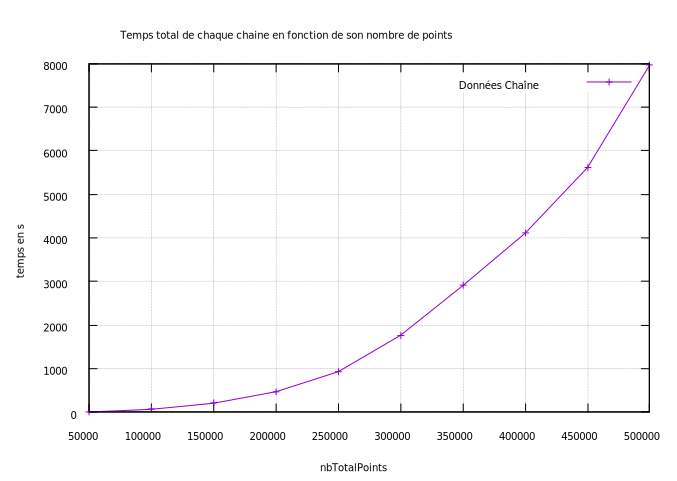
\includegraphics[width=0.85\linewidth]{comparaison/graphChaines.png}} % Insère l'image dans un cadre
  \captionsetup{justification=centering} % Centrer la légende
  \caption{Évolution des \textbf{temps d'exécution} de la liste chaînée \\ en fonction du \textbf{nombre de points} (pas de 500)} % Ajoute une légende à l'image
  \label{fig:exemple} % Ajoute une étiquette pour faire référence à l'image
\end{figure}
\end{center}

% Graphique 2
\begin{center}
\begin{figure} % "h" spécifie que l'image doit être placée ici si possible
  \centering % Centre l'image
  \fbox{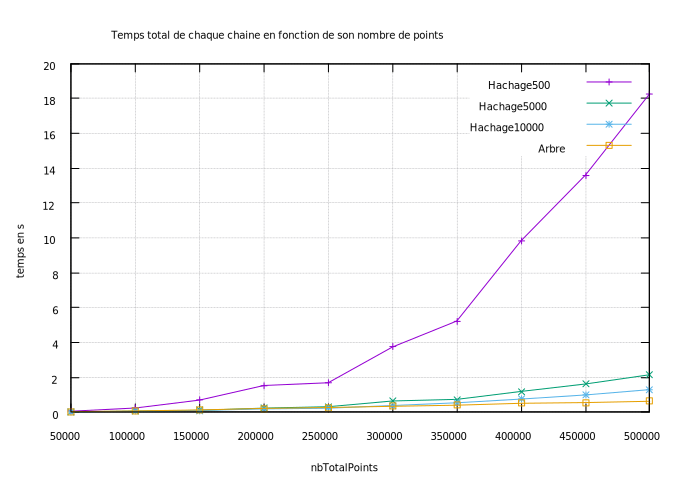
\includegraphics[width=0.85\linewidth]{comparaison/graphGlob.png}} % Insère l'image dans un cadre
  \captionsetup{justification=centering} % Centrer la légende
  \caption{Evolution des \textbf{temps dexécution} de la \textbf{Table de Hachage} de taille 5000, 50000 et de \textbf{Arbre Quaternaire} en fonction du \textbf{nombre de points} (pas de 500)} % Ajoute une légende à l'image
  \label{fig:exemple} % Ajoute une étiquette pour faire référence à l'image
\end{figure}
\end{center} 

% Graphique 3
\begin{center}
\begin{figure} % "h" spécifie que l'image doit être placée ici si possible
  \centering % Centre l'image
  \fbox{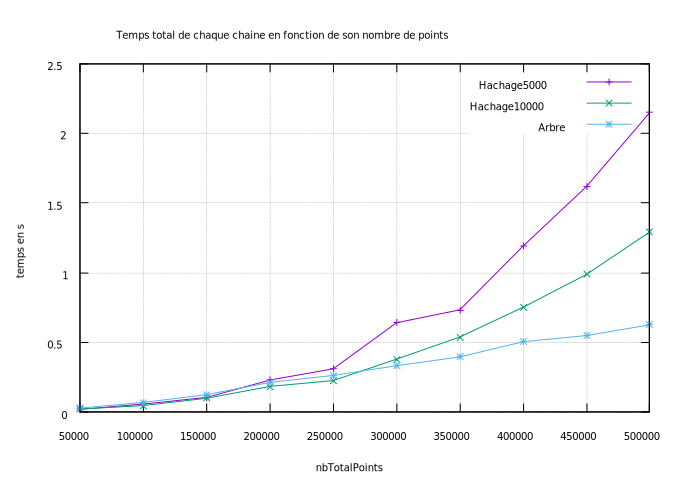
\includegraphics[width=0.85\linewidth]{comparaison/graphDetail.png}} % Insère l'image dans un cadre
  \captionsetup{justification=centering} % Centrer la légende
  \caption{Évolution des \textbf{temps d'exécution} de la \textbf{Table de Hachage} de taille 500, 5000, 50000 et de \textbf{Arbre Quaternaire} en fonction du \textbf{nombre de points} (pas de 500)} % Ajoute une légende à l'image
  \label{fig:exemple} % Ajoute une étiquette pour faire référence à l'image
\end{figure}
\end{center} 



\subsection*{Question 4}
\addcontentsline{toc}{subsection}{Question 4}

En comparant la figure 1 et 2, on peut remarquer que la reconstitution à partir de listes chaînées est beaucoup plus longue que les autres.
\\ \\ 
Cela s'explique par le fait que la \textbf{complexité de la chaîne} est en \textbf{O(nxm)}. En effet, la chaîne est composée de listes chaînées qui contiennent elle mêmes des listes chaînées. Ainsi, la complexité de la chaîne est en O(nxm), avec n le \textbf{nombre de chaînes} et m le \textbf{nombre de points} dans les chaînes. Ces deux valeurs sont variables. 
\\ \\ \\
En regardant la figure 2 et 3, on peut analyser les performances du Hachage ainsi que de l'arbre.
\\ \\ 
Plus la \textbf{table de hachage} est grande, plus les temps d'exécution sont courts. Cela est aussi à la complexité de la table de hachage. Sa complexité dépend de sa \textbf{taille} ainsi que du \textbf{nombre d'éléments} à ajouter. Plus la table est grande, moins il y a de \textbf{collisions} à gérer. Par exemple, pour une table de taille 1, on aura seulement une liste chaînée. On devra alors la parcourir en entier, ce qui revient à une complexité de n (nb éléments dans la liste). A l'inverse pour une table plus grande que le nombre d'éléments qu'elle contient et avec une fonction de hachage qui réparti bien les éléments, on aura une \textbf{complexité de 1} (omega(1)).
\\ \\
Sur la figure 3, on se rend aussi compte que l'arbre a un temps d'exécution plus \textbf{rapide que les autres}, peu importe le nombre de points total qu'on lui donne. Cela est aussi dû à sa \textbf{complexité en log4(n)}. A chaque fois que l'on cherche un point, on sait dans \textbf{quelle branche de l'arbre} regarder. On arrive donc très rapidement à trouver ou non le noeud recherché.


\end{document}
